\documentclass[a4paper,11pt]{article}
\usepackage[utf8]{inputenc}
\usepackage{amsmath}
\usepackage{amsfonts}
\usepackage{amssymb}
\usepackage{graphicx}
\usepackage{braket}

\numberwithin{equation}{section}
\renewcommand\thesubsection{\alph{subsection}}
\newcommand{\bvp}[1]{\mathbf{#1}'}
\newcommand{\bv}[1]{\mathbf{#1}}
\newcommand{\pp}[1]{#1'}


%opening
\title{Quantum III HW2}
\author{Vince Baker}

\begin{document}

\maketitle

\section{Problem 1}
We first examine the inner product $\braket{\psi_n|W|\psi_i}$, using the ladder operator relation $\hat{X}=\sqrt{\frac{\hbar}{2m\omega}}(a+a^\dagger)$.
\begin{align}
 \braket{\psi_n|W|\psi_i} &= -qE\sqrt{\frac{\hbar}{2m\omega}}\braket{\psi_n|(a+a^\dagger)|\psi_n}\\
 \braket{\psi_n|W|\psi_i} &= -qE\sqrt{\frac{\hbar}{2m\omega}}(\braket{\psi_n|\psi_{i-1}}+\braket{\psi_n|\psi_{i+1}} )\\
 \braket{\psi_n|W|\psi_i} &= -qE\sqrt{\frac{\hbar}{2m\omega}}(\delta_{n,n-1}+\delta_{n,n+1})
\end{align}
a) We examine the first-order perturbation theory result for $C_{10}$:
\begin{align}
 C_{01}^1 &= -\frac{i}{\hbar}\int_0^t dt^\prime e^{i\omega_{10}t^\prime}\braket{\psi_1|W|\psi_0}\\
 C_{01}^1 &= qE\sqrt{\frac{\hbar}{2m\omega_0}}\frac{1}{E_1-E_0}\left(e^{\frac{i}{\hbar}(E_1-E_0)\tau}-1 \right)\\
 C_{01}^1 &= qE\sqrt{\frac{1}{2m\hbar\omega_0^3}}\left(e^{i\omega_0\tau}-1 \right)\\
 |C_{01}^1|^2 &= \frac{(qE)^2}{2m\hbar\omega_0^3} \left(2-(e^{i\omega_0\tau}+e^{-i\omega_0\tau} \right)\\
 |C_{01}^1|^2 &= \frac{(qE)^2}{m\hbar\omega_0^3}\left(1-\cos{\omega_0\tau} \right)
\end{align}
The probabiltiy varies at the harmonic ocsillator amgular frequency.\\
\\
b) We now examine $C_{20}$. We have seen that $\braket{\psi_2|W|\psi_0}=0$, so the first-order approximation will be 0.
For the second-order perturbation results, $\braket{\psi_2|W|\psi_1}=\braket{\psi_1|W|\psi_0}=-qE\sqrt{\frac{\hbar}{2m\omega}}$.
So only the transition through intermediate state $\ket{1}$ will contribute.
\begin{align}
 C_{01}^2 &= -\frac{1}{\hbar^2}\int_0^\tau dt^\prime e^{i\omega_{21}t^\prime}W_{21}\int_0^{t\prime}dt^{\prime}e^{i\omega_{10}t^\prime}W_{10}\\
 C_{01}^2 &= \frac{iq^2E^2}{2m\omega_0^2\hbar}\int_0^\tau dt^\prime e^{i2\omega_0t^\prime}-e^{i\omega_0 t^\prime}\\
 C_{01}^2 &= \frac{q^2E^2}{2m\omega_0^3\hbar}\left(\frac{e^{i2\omega_0\tau}-1}{2}-e^{i\omega_0\tau}+1 \right)\\
 C_{01}^2 &= \frac{q^2E^2}{4m\omega_0^3\hbar}\left(e^{i\omega_0\tau}-1 \right)^2\\
 |C_{01}^2|^2 &= \left(\frac{q^2E^2}{4m\omega_0^3\hbar}\right)^2\left(e^{i\omega_0\tau}-1 \right)^2\\
 |C_{01}^2|^2 &= \left(\frac{q^2E^2}{4m\omega_0^3\hbar}\right)^2
		 \left(e^{i2\omega_0\tau}+e^{-i2\omega_0\tau}-4(e^{i\omega_0\tau}+e^{-i\omega_0\tau})+6 \right)\\
 |C_{01}^2|^2 &= \left(\frac{q^2E^2}{4m\omega_0^3\hbar}\right)^2 \left(2\cos{2\omega_0\tau}-8\cos{\omega_0\tau}+6\right)
\end{align}
A scaled version of this function is plotted below. The probability again oscillates at the harmoic oscillator frequency $\omega_0$.
\\
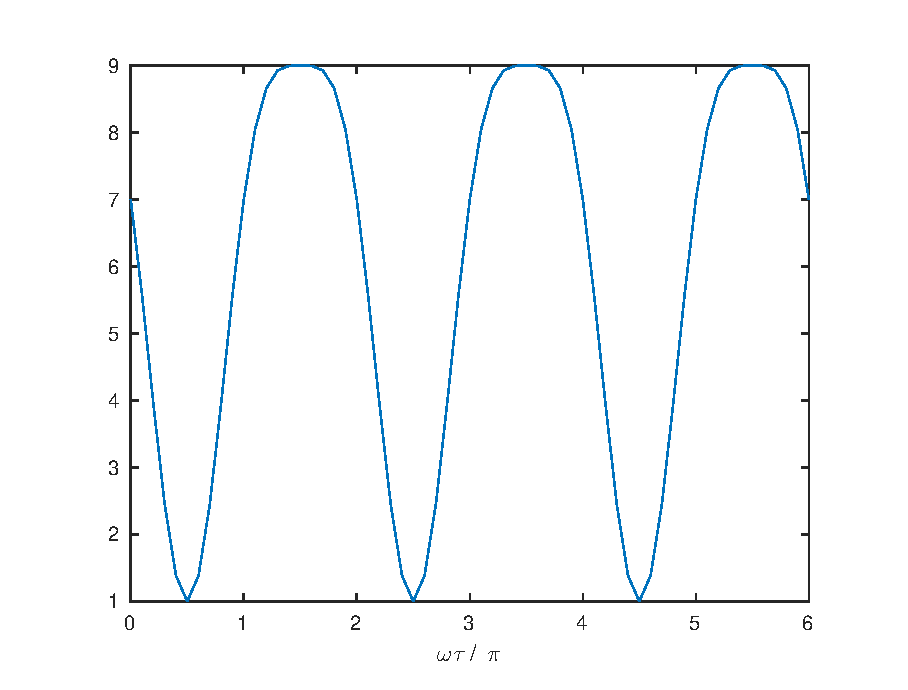
\includegraphics{p1_b}
\\
\section{Problem 2}
Wigner and Weisskopf analyze a time-dependent perturbation of a stationary system in the interaction picture. 
They find an energy shift as well as a line broadening using second-order results.
Fano found the stationary states of a system with an interaction potential between a discrete state and a comtinuum of states using the Schrodinger picture. 
Fano's exact result using the Schordinger picture determines that the discrete state is diluted across a range of continuum states near the discrete-state energy.\\
If we consider the discrete-continuum interaction terms in the Hamiltonian as a time-dependent perturbation we can view the Wigner-Weisskopf results as an approximation of Fano's results.
However, the time-dependent perturbation results as presented by Wigner-Weisskopf has a decay width term:
\begin{align}
 \Gamma &= 2\pi\sum_{m \ne i}|V_{mi}|^2\delta(E_i-E_m)
\end{align}
Unlike Fano's result, there is no sudden phase change as the continuum energy passes through the discrete state energy, so Wigner-Weisskopf does not predict the asymmetric absorption peaks that Fano explained.
\section{Problem 3}
We follow Fano's derivation of the factorization:
\begin{align}
 \begin{split}
 \frac{1}{(\bar{E}-\pp{E})(E-\pp{E})} = &\frac{1}{\bar{E}-\pp{E}}\left(\frac{1}{E-\pp{E}}-\frac{1}{\bar{E}-\pp{E}} \right)\\
				      &+\pi^2\delta(\bar{E}-E)\delta(\pp{E}-\frac{1}{2}(\bar{E}+E))
 \end{split}
\end{align}
We begin by determing the Fourier expansion of $\frac{1}{E-\pp{E}}$.
\begin{align}
 \frac{1}{E-\pp{E}} &= \int_{-\infty}^\infty\hat{f}(k)e^{i2\pi k\pp{E}}dk\\
 \hat{f}(k) &= \int_{-\infty}^\infty \frac{1}{E-\pp{E}}e^{-i2\pi k\pp{E}}d\pp{E}
\end{align}
We evaluate 3.3 with its single pole using the residue theorem. 
When $k>0$ we will close the contour in the upper half of the complex plane, and we will avoid the pole using a counter-clockwise circle. 
When $k<0$ we will close the contour in the lower half of the complex plane, and we will avoid the pole using a clockwise circle.
This leads to:
\begin{align}
 P(\int) -i\pi Res = 0 \ (k<0)\\
 P(\int) +i\pi Res = 0 \ (k>0)
\end{align}
The residue at the simple pole can be evaluated using $lim(\pp{E} \rightarrow E)(E-\pp{E})\frac{ e^{-i2\pi k\pp{E}} }{E-\pp{E}}=e^{-i2\pi kE}$.
Writing the sign of k as $\frac{k}{|k|}$, and noting that $ie^{i\theta}=e^{-i\theta}$, we have proved Fano's equation A1:
\begin{align}
 \frac{1}{E-\pp{E}} &= -i\pi\int_{-\infty}^\infty \frac{k}{|k|}e^{i2\pi k(E-\pp{E})}dk
\end{align}
We can now write the double-pole expression as:
\begin{align}
 \frac{1}{(\bar{E}-\pp{E})(E-\pp{E})} &= -\pi^2\int_{-\infty}^\infty dk \int_{-\infty}^\infty d\pp{k}
	      \frac{k\pp{k}}{|k\pp{k}|}e^{i2\pi [ k(\bar{E}-\pp{E})+\pp{k}(E-\pp{E})]}
\end{align}
Fano now makes the substitution $u=k+\pp{k},\ v=\frac{1}{2}(k-\pp{k})$ and finds that:
\begin{align}
 u^2 &= k^2+2k\pp{k}+\pp{k}^2\\
 4v^2 &= k^2-2k\pp{k}+\pp{k}^2\\
 \frac{k\pp{k}}{|k\pp{k}|} &= \frac{u^2-4v^2}{|u^2-4v^2|}
\end{align}
This expression will be -1 for $u^2<4v^2$ and +1 for $u^2>4v^2$, so it is equivalent to  $2St(u^2-4v^2)-1$ where $St()$ is the step function.
This substitution allows us to write equation7 as:
\begin{align}
  \begin{split}
  \frac{1}{(\bar{E}-\pp{E})(E-\pp{E})} = &\pi^2 \int_{-\infty}^\infty du\ e^{i2\pi u[\frac{1}{2}(\bar{E}+E)-\pp{E}) ]} \\
					&\times \left( \int_{-\infty}^\infty\ dv-2\int_{-\frac{1}{2}|u|}^{\frac{1}{2}|u|}\ dv \right) e^{i2\pi v(\bar{E}-E)}
  \end{split}
\end{align}
Using the exponential delta function $\delta(x-a) = \int e^{x-a}dx$
\\
\section{Problem 4}
We start from Fano eq. 10:
\begin{align}
 \begin{split}
 a^*(\bar{E})\{1+\int d\pp{E} V_{\pp{E}}^*
	    &\left(\frac{1}{\bar{E}-\pp{E}}+z(\bar{E})\delta(\bar{E}-\pp{E}\right)\\
	    &\times \left(\frac{1}{E-\pp{E}}+z(E)\delta(E-\pp{E})\right)V_{\pp{E}} \}a(E)\\
	    &= \delta(\bar{E}-E) 
 \end{split}	    
\end{align}
Opening up the expression under the integral we find:
\begin{align}
 \begin{split}
  a^*(\bar{E})a(E)\{1&+\int |V_{\pp{E}}|^2\frac{1}{(\bar{E}-\pp{E})(E-\pp{E})} d\pp{E}\\
	      &+\int |V_{\pp{E}}|^2\frac{z(\bar{E})\delta(\bar{E}-\pp{E})}{\bar{E}-\pp{E}}d\pp{E}\\
	      &+\int |V_{\pp{E}}|^2\frac{z(E)\delta(E-\pp{E})}{E-\pp{E}}    d\pp{E}\\
	      &+\int |V_{\pp{E}}|^2 z(\bar{E})z(E)\delta(\bar{E}-\pp{E})\delta(E-\pp{E})   d\pp{E}\\
	      &= \delta(\bar{E}-E) 
 \end{split}
\end{align}
The first expression is expanded using the result of problem 3 and the definition of $F(E)=P\int d\pp{E} \frac{|V_{\pp{e}}|^2}{E-\pp{E}}$.
\begin{align}
 \begin{split}
  \int |V_{\pp{E}}|^2\frac{1}{(\bar{E}-\pp{E})(E-\pp{E})} d\pp{E} &= \frac{|V_E|^2}{\bar{E}-E}\left(F(E)-F(\bar{E}) \right)\\
			  &+\pi^2\delta(\bar{E}-E)
 \end{split}
\end{align}
The second and third expressions in 4.2 can be combined into $\frac{1}{\bar{E}-E}\left(z(E)|V_E^2-z(\bar{E})|V_{\bar{E}}|^2 \right)$.
\\
Using $\delta(\bar{E}-\pp{E})\delta(E-\pp{E})=\delta(\bar{E}-E)\delta(\pp{E}-\frac{1}{2}(\bar{E}+E))$ the fourth expression is:
\begin{align}
 \int |V_{\pp{E}}|^2 z(\bar{E})z(E)\delta(\bar{E}-\pp{E})\delta(E-\pp{E}) d\pp{E} &= |V_{E}|^2 z(E)^2\delta(\bar{E}-E)
\end{align}
We can now collect terms:
\begin{align}
 \begin{split}
  |a(E)|^2&|V_E|^2(\pi^2+z(E)^2)\delta(\bar{E}-E)+a^*(\bar{E})a(E)\\
      &\times\left\{1+\frac{1}{\bar{E}-E}\left(F(E)-F(\bar{E})
         +z(E)|V_E|^2-z(\bar{E})|V_{\bar{E}}|^2  \right) \right\}\\
         &=\delta(\bar{E}-E)
 \end{split}
\end{align}
Since $F(E)=E-z(E)|V_E|^2-E_\phi$, the term inside the brackets reduces to $1+\frac{E-\bar{E}}{\bar{E}-E}=0$ so the second term vanishes.
We then have:
\begin{align}
 |a(E)|^2 =\frac{1}{|V_E|^2(\pi^2+z(E)^2)}=\frac{|V_E|^2}{(E-E_\phi-F(E))^2+\pi^2|V_E|^4}
\end{align}
\\
\section{Problem 5}




\end{document}
